%% Manuscript for Computer Methods and Programs in Biomedicine (Elsevier), elsarticle class.
%% Compile: tectonic main.tex   (or pdflatex + bibtex + pdflatex x2, or upload the folder to Overleaf)
\documentclass[preprint,12pt]{elsarticle}

\usepackage{amsmath,amssymb}
\usepackage{graphicx}
\usepackage{booktabs}
\usepackage{array}
\usepackage{tabularx}
\usepackage{multirow}
\usepackage[hidelinks]{hyperref}
\usepackage{xurl}
\usepackage{tikz}
\usetikzlibrary{arrows.meta,positioning,fit,backgrounds}

\setlength{\emergencystretch}{1.5em}
\newcolumntype{Y}{>{\raggedright\arraybackslash}X}
\newcommand{\figfile}[2]{\IfFileExists{#1}{\includegraphics[width=#2]{#1}}{\fbox{\parbox{0.8\linewidth}{\centering\vspace{2cm}Missing file: \texttt{\detokenize{#1}}\vspace{2cm}}}}}

\journal{Computer Methods and Programs in Biomedicine}

\begin{document}

\begin{frontmatter}

\title{Recognising the phone, not the throat: deconfounded evaluation and shortcut mitigation for smartphone pharyngitis classification}

\author[a]{Sandesh Bhatta\corref{cor1}}
\ead{sbhatta@albany.edu}
\ead[url]{https://orcid.org/0009-0008-0399-0480}
\cortext[cor1]{Corresponding author.}

\affiliation[a]{organization={Department of Computer Science, University at Albany, State University of New York},
            city={Albany},
            state={New York},
            country={USA}}

\begin{abstract}
\textit{Background and Objective:} Smartphone throat photographs could help separate bacterial from non-bacterial pharyngitis. On the public PGUPharyngitis dataset (742 patients, two cities, one phone model per city), image models reach AUCs near 0.65--0.70, but bacterial prevalence differs threefold between the two phones. We asked how much of this performance comes from recognising the phone, how to measure performance without that shortcut, and whether standard mitigation methods recover a device-independent signal.

\textit{Methods:} We analysed 735 patients with physician-consensus labels in 5-fold cross-validation repeated five times with nested tuning. We benchmarked symptom models, frozen and fine-tuned image networks and five fusion methods, and audited them with phone-only and photo-statistics baselines, phone identification, and within- and cross-phone evaluation. We introduce a deconfounded AUC that reweights patients so the label is independent of the phone; any phone-only predictor scores 0.5. We then compared 13 mitigation variants on two backbones: colour constancy, per-phone standardisation, linear concept erasure (LEACE), reweighting, covariate adjustment and adversarial training, each with a probe that measures how much phone information remains.

\textit{Results:} The best pooled AUC was 0.703 (stacked image--symptom fusion); the phone alone reached 0.673, and image features identified the phone with AUC 0.99. Deconfounded AUCs of image, symptom and fusion models were 0.52--0.58 (DINOv2 image 0.558, 95\% CI 0.51--0.61; phone only 0.496). The 0.11 pooled-AUC advantage of images over symptoms ($p < 0.001$) shrank to 0.01 ($p = 0.75$). Per-phone standardisation and LEACE removed phone information (probe AUC from 0.99 to 0.51--0.52) and lowered pooled AUC to 0.54--0.58, but no method changed deconfounded AUC (all $p > 0.19$). Adversarial training lowered pooled AUC while the phone stayed identifiable (probe AUC 0.97--0.98).

\textit{Conclusions:} Most of the apparent image performance on PGUPharyngitis is a device shortcut, and removing it reveals a weak signal (AUC about 0.56) that current mitigation methods do not improve. Deconfounded AUC, phone-only baselines and leakage probes should be reported for multi-site smartphone imaging models.
\end{abstract}

\begin{graphicalabstract}
\figfile{figures/graphical_abstract.png}{\textwidth}
\end{graphicalabstract}

\begin{highlights}
\item The phone model alone predicts expert pharyngitis labels with AUC 0.67.
\item A deconfounded AUC, under which any phone-only model scores 0.5, is introduced.
\item Deconfounded, image and fusion models fall from about 0.70 to 0.52--0.58.
\item Concept erasure removes the phone signal but recovers no throat signal.
\item Adversarial debiasing lowers AUC yet leaves the phone 97\% identifiable.
\end{highlights}

\begin{keyword}
shortcut learning \sep confounding \sep smartphone imaging \sep pharyngitis \sep concept erasure \sep deep learning
\end{keyword}

\end{frontmatter}


%% ---------------------------------------------------------------------------------------------
\section{Introduction}
\label{sec:intro}

Sore throat is one of the most common reasons for primary-care visits, and most cases are viral. Group A streptococcus and other bacteria cause a minority of cases, yet antibiotics are prescribed far more often than bacterial infection occurs \cite{shulman2012idsa,spinks2021cochrane}. Clinical scores such as Centor and McIsaac combine fever, tonsillar exudate, tender cervical lymph nodes, absence of cough and age to estimate the probability of streptococcal infection \cite{centor1981,mcisaac1998}. They are simple and widely taught, but their discrimination is moderate and they depend on a careful physical examination.

Smartphone photographs of the throat are a cheap alternative that also works remotely. Deep-learning models trained on such photographs have detected severe pharyngitis \cite{yoo2020pharyngitis} and streptococcal pharyngitis \cite{askarian2019strep} in small single-site studies. In 2025, Shojaei et al.\ released PGUPharyngitis, the largest public dataset of its kind: 742 throat photographs from patients with cold symptoms in two Iranian cities, taken with two phone models, each labelled bacterial or non-bacterial by four to nine physicians, together with 20 symptoms, age and sex \cite{shojaei2025pgu}. Their image-only baselines reached an AUC of 0.645 (DenseNet121), and the dataset was offered to support AI-based diagnosis and remote care. The intended users of such a model are primary-care and telemedicine clinicians deciding whether a sore throat is likely to be bacterial. Streptococcal pharyngitis is most common in school-age children \cite{shulman2012idsa}, so performance should be checked across age groups.

Two questions remain open. First, the dataset records symptoms, and physicians labelled each case from the photograph and the symptoms together, yet no published model combines the two. Multimodal fusion of images with clinical variables often improves medical prediction \cite{huang2020fusion}, so fusion is worth testing here. Second, nobody has checked what image models learn on this dataset. Deep networks readily exploit ``shortcuts'': features that predict the label in the training data but are unrelated to the disease \cite{geirhos2020shortcut}. In chest radiography, models identified the hospital and scanner and used them to predict pneumonia or COVID-19 \cite{zech2018pneumonia,degrave2021covid}, and hip-fracture models leaned on scanner and patient variables \cite{badgeley2019hip}. In PGUPharyngitis, each city used a different phone, and bacterial prevalence may differ between cities. A model could therefore score well by recognising the phone.

We set out to build a symptom-aware image model and found that pooled cross-validation on this dataset mostly measures how well a model recognises the phone. Showing that a shortcut exists is only the first step, and it leaves two practical questions for anyone working with multi-site smartphone images. How should a model be scored so that the shortcut earns no credit? And can standard debiasing methods remove the shortcut while keeping a real throat signal? Within-site AUC answers the first question only partly: it discards every comparison between sites and becomes unstable when one site has few positive cases. Mitigation methods from the fairness and domain-adaptation literature (colour constancy, feature harmonisation, concept erasure, reweighting and adversarial training) are rarely compared on the same medical data, and their success is usually judged by pooled accuracy, which a shortcut inflates.

This study makes four contributions:
\begin{enumerate}
\item \textit{A shortcut audit of PGUPharyngitis.} The phone alone, or 18 global colour statistics, match the published image baseline; image features identify the phone almost perfectly; and image performance largely disappears within a phone and across phones.
\item \textit{A deconfounded AUC.} Weighting each patient by $P(y)/P(y \mid \text{site})$ makes the label independent of the site, so any predictor that uses only the site scores 0.5, while comparisons between patients from different sites are kept. Under this metric the 0.11 AUC advantage of images over symptoms disappears.
\item \textit{A controlled comparison of shortcut mitigation.} Thirteen variants of six method families were tested on two backbones under the same nested protocol, each with a probe of how much phone information remains. Methods that remove the phone signal lower the pooled AUC to the deconfounded level but do not raise the deconfounded AUC, and adversarial training gives a misleading impression of success.
\item \textit{A multimodal benchmark with open code.} Symptom-only, image-only, clinical-score and five fusion approaches, including a gated cross-modal network, are compared under one repeated, nested cross-validation protocol. Code, folds and out-of-fold predictions are released so that future work can report the same metrics.
\end{enumerate}

%% ---------------------------------------------------------------------------------------------
\section{Related work}
\label{sec:related}

\paragraph{Clinical scores} The Centor score assigns one point each for fever, tonsillar exudate, tender anterior cervical lymphadenopathy and absence of cough \cite{centor1981}; McIsaac added an age adjustment \cite{mcisaac1998}. Both are used to decide on testing or empirical antibiotics, and both need findings from a physical examination. PGUPharyngitis records fever and cough but not exudate or lymph nodes, so only a modified score can be computed.

\paragraph{Throat-image AI} Yoo et al.\ trained convolutional networks on smartphone throat photographs to separate severe pharyngitis from normal throats \cite{yoo2020pharyngitis}, and Askarian et al.\ used colour and texture features from smartphone images to detect streptococcal pharyngitis \cite{askarian2019strep}. These studies were small and from single sites. Shojaei et al.\ released PGUPharyngitis with image-only baselines evaluated by three-fold cross-validation, reporting AUCs from 0.554 (MobileNetV3) to 0.645 (DenseNet121) on the full dataset \cite{shojaei2025pgu}. To our knowledge, no study has fused these images with symptoms or examined what the models learn.

\paragraph{Multimodal fusion} Medical image--tabular fusion is usually grouped into early fusion (concatenating features), late fusion (combining predictions) and joint or intermediate fusion (learning a shared representation) \cite{huang2020fusion}. Gated units learn how much to trust each modality per sample \cite{arevalo2017gmu}, and feature-wise linear modulation (FiLM) lets one modality scale and shift the features of another \cite{perez2018film}. We implement all of these families on equal terms.

\paragraph{Shortcut learning and site confounding} Shortcut learning occurs when a model relies on cues that are predictive in the training distribution but not causally related to the target \cite{geirhos2020shortcut}. In medical imaging, such cues include the hospital, scanner, positioning markers and patient metadata \cite{zech2018pneumonia,degrave2021covid,badgeley2019hip}. Hidden stratification, where performance is driven by an easy subgroup, can make overall metrics misleading \cite{oakdenrayner2020hidden}. Methodological reviews recommend evaluation across sites, explicit confounder baselines and reporting of variance across splits \cite{varoquaux2022failures}. Brown et al.\ proposed testing whether a model's reliance on a sensitive attribute changes its fairness \cite{brown2023shortcut}, and Ong Ly et al.\ showed that shortcut learning lowers performance on external data and proposed estimating generalisation without it \cite{ongly2024shortcut}. We apply these recommendations to throat imaging.

\paragraph{Shortcut mitigation} Methods for removing an unwanted attribute fall into a few families. Colour constancy normalises the illuminant and camera colour cast of each image; Shades of Gray \cite{finlayson2004shades} improved dermoscopy classification across acquisition conditions \cite{barata2015colour}. Feature harmonisation removes site-specific location and scale, as ComBat does for batch effects \cite{johnson2007combat}. Linear concept erasure removes all linearly available information about an attribute; LEACE does so in closed form with the smallest possible change to the features \cite{belrose2023leace}. Reweighting or resampling the training data so that label and nuisance are independent targets the shortcut directly \cite{makar2022causally}. Adversarial training with a gradient-reversal layer penalises representations from which the domain can be predicted \cite{ganin2016dann}, although in text data the removed attribute could still be recovered from the learned representation \cite{elazar2018adversarial}. We compare these families on the same data and measure how much site information each leaves behind.

%% ---------------------------------------------------------------------------------------------
\section{Materials and methods}
\label{sec:methods}

The study is reported following TRIPOD+AI \cite{collins2024tripodai}. All analyses are exploratory: the analysis plan was written before modelling, but hypotheses were not formally frozen before the first results were seen. Figure~\ref{fig:design} summarises the study design.

\begin{figure}[!htbp]
\centering
\IfFileExists{figures/fig1_study_design.pdf}{\includegraphics[width=\textwidth]{figures/fig1_study_design.pdf}}{%
\resizebox{\textwidth}{!}{%
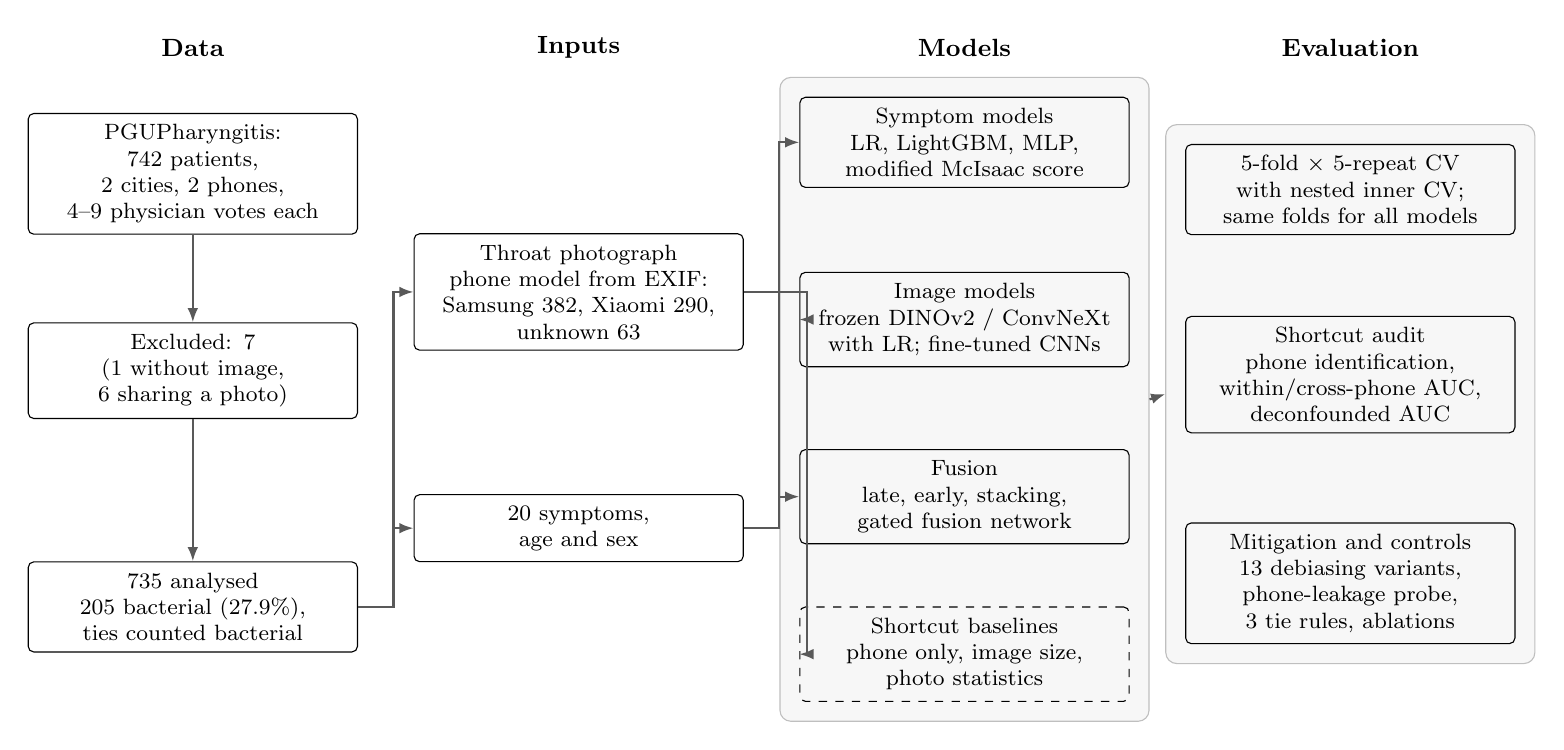
\begin{tikzpicture}[
  font=\footnotesize,
  box/.style={draw, rounded corners=2pt, align=center, text width=3.9cm, inner sep=4pt},
  base/.style={box, dashed},
  hdr/.style={font=\small\bfseries},
  arr/.style={-{Latex[length=1.8mm]}, thick, gray!70!black}]
% column headers
\node[hdr] at (0,2.2) {Data};
\node[hdr] at (4.9,2.2) {Inputs};
\node[hdr] at (9.8,2.2) {Models};
\node[hdr] at (14.7,2.2) {Evaluation};
% data
\node[box] (d1) at (0,0.6) {PGUPharyngitis: 742 patients,\\2 cities, 2 phones,\\4--9 physician votes each};
\node[box] (d2) at (0,-1.9) {Excluded: 7\\(1 without image,\\6 sharing a photo)};
\node[box] (d3) at (0,-4.9) {735 analysed\\205 bacterial (27.9\%),\\ties counted bacterial};
\draw[arr] (d1) -- (d2);
\draw[arr] (d2) -- (d3);
% inputs
\node[box] (i1) at (4.9,-0.9) {Throat photograph\\phone model from EXIF:\\Samsung 382, Xiaomi 290,\\unknown 63};
\node[box] (i2) at (4.9,-3.9) {20 symptoms,\\age and sex};
\draw[arr] (d3.east) -- ++(0.45,0) |- (i1.west);
\draw[arr] (d3.east) -- ++(0.45,0) |- (i2.west);
% models
\node[box] (m1) at (9.8,1.0) {Symptom models\\LR, LightGBM, MLP,\\modified McIsaac score};
\node[box] (m2) at (9.8,-1.25) {Image models\\frozen DINOv2 / ConvNeXt\\with LR; fine-tuned CNNs};
\node[box] (m3) at (9.8,-3.5) {Fusion\\late, early, stacking,\\gated fusion network};
\node[base] (m4) at (9.8,-5.5) {Shortcut baselines\\phone only, image size,\\photo statistics};
\draw[arr] (i2.east) -- ++(0.45,0) |- (m1.west);
\draw[arr] (i2.east) -- ++(0.45,0) |- (m3.west);
\draw[arr] (i1.east) -- ++(0.8,0) |- (m2.west);
\draw[arr] (i1.east) -- ++(0.8,0) |- (m4.west);
% evaluation
\node[box] (e1) at (14.7,0.4) {5-fold $\times$ 5-repeat CV\\with nested inner CV;\\same folds for all models};
\node[box] (e2) at (14.7,-1.95) {Shortcut audit\\phone identification,\\within/cross-phone AUC,\\deconfounded AUC};
\node[box] (e3) at (14.7,-4.6) {Mitigation and controls\\13 debiasing variants,\\phone-leakage probe,\\3 tie rules, ablations};
\begin{scope}[on background layer]
  \node[draw=gray!50, fill=gray!6, rounded corners=4pt, inner sep=7pt, fit=(m1)(m4)] (M) {};
  \node[draw=gray!50, fill=gray!6, rounded corners=4pt, inner sep=7pt, fit=(e1)(e3)] (E) {};
\end{scope}
\draw[arr] (M.east) -- (E.west);
\end{tikzpicture}}}
\caption{Study design: 742 patients, 735 analysed; inputs (photograph, 20 symptoms, age, sex), model families, 5\,$\times$\,5 nested cross-validation, the shortcut audit and the mitigation experiments.}
\label{fig:design}
\end{figure}

\subsection{Dataset}

We used PGUPharyngitis (Figshare, \url{https://doi.org/10.6084/m9.figshare.28163513}, CC BY 4.0) \cite{shojaei2025pgu}. It contains one throat photograph per patient, taken with a Samsung Galaxy S21 Ultra or a Xiaomi phone in two Iranian cities between October 2023 and May 2024, and a table with age, sex, 20 binary symptoms and four to nine physician diagnoses (bacterial or non-bacterial). The original study received ethics approval (IR.BPUMS.REC.1403.282) with written informed consent; we used the anonymised public release only.

The table lists 742 patients. Patient 666 had no image. Three pairs of patients (19/23, 218/256, 301/305) shared an identical photograph (perceptual-hash distance 0) but had different ages, sexes or symptoms; because the image could not be assigned to either record, we excluded all six. The analysis set has 735 patients. The table has no city or phone column, so we read the phone model from each photograph's EXIF metadata: Samsung (model code SM-G998B) for 382 patients, Xiaomi (2201117SG) for 290, and unknown for 63. Because each city used one phone \cite{shojaei2025pgu}, we treat the phone as a proxy for acquisition site and write ``phone/site'' throughout. Treatments were not recorded. The sample size was fixed by the public dataset and no sample size calculation was done; with 205 bacterial cases, AUC confidence intervals are about $\pm 0.04$ wide, and we report them throughout.

\subsection{Labels}

The 735 patients received 3,662 diagnoses (median 5 per patient; one patient had 3 recorded). The reference label is the majority vote. One hundred patients (13.6\%) had a tied vote; in the primary analysis ties count as bacterial, giving 205 bacterial cases (27.9\%). Two sensitivity analyses count ties as non-bacterial (105 bacterial, 14.3\%) or exclude them (635 patients, 16.5\% bacterial). We also keep the soft label, the share of physicians voting bacterial, and the agreement, $|\text{soft} - 0.5| \times 2$; 230 patients (31\%) had unanimous votes. The labels reflect expert consensus from photographs and symptoms, not microbiological testing. The data paper does not report the physicians' specialties or whether they were blinded to each other's diagnoses \cite{shojaei2025pgu}.

\subsection{Preprocessing}

Images were rotated according to EXIF orientation, converted to RGB and resized so the short side was 256 pixels. Training augmentation used a random resized crop to $224 \times 224$ (scale 0.8--1.0), horizontal flip, rotation up to $15^\circ$ and brightness and contrast jitter of 10\%. Hue and saturation were not altered, because throat redness is diagnostic. At test time we used a 224-pixel centre crop and averaged predictions over the original and a horizontally flipped image. Images were normalised with ImageNet statistics. Tabular inputs were the 20 symptoms, sex (0/1) and age; age was standardised and any missing value imputed using statistics from the training data only (no values were missing).

\subsection{Evaluation protocol}

All models used the same stratified 5-fold cross-validation repeated five times with different seeds (25 test folds of 147 patients), stratified on label $\times$ phone. Fold assignments are released with the code. Within each training part, a 3-fold inner cross-validation selected hyperparameters (by AUC), the number of training epochs for neural fusion models, and the decision threshold, chosen to maximise balanced accuracy on inner out-of-fold predictions. Scalers, imputers, PCA, thresholds and stacking meta-models were fitted on training data only. Because fine-tuning is costly, fine-tuned CNNs used one repeat (5 folds) and a stratified 15\% validation split of each training part for early stopping and threshold choice.

\subsection{Models}

\paragraph{Symptom models} Logistic regression (L2, class-balanced, $C \in \{0.01, 0.1, 1, 10\}$), LightGBM \cite{ke2017lightgbm} (4 or 8 leaves, 100 or 300 trees, learning rate 0.05) and a two-layer perceptron (64--64 units, L2 penalty $\in \{0.001, 0.1, 1\}$) used the 20 symptoms, sex and age.

\paragraph{Clinical score} A modified McIsaac score summed fever (``Pyrexia''), absence of cough and an age term ($+1$ for 3--14 years, $-1$ for $\geq 45$ years) \cite{mcisaac1998}; exudate and lymph-node items are not recorded.

\paragraph{Reference baselines} To measure shortcuts we trained three models that do not use throat anatomy: (i) \textit{phone only}, predicting the training-fold bacterial rate of the photograph's phone; (ii) \textit{image size}, logistic regression on the log width, height, aspect ratio and area of the original photograph; and (iii) \textit{photo statistics}, logistic regression on 18 global statistics of each resized photograph (RGB and HSV means and standard deviations, shares of dark, bright and strongly red pixels, and edge density).

\paragraph{Frozen image models} We extracted embeddings from DINOv2 ViT-S/14 \cite{oquab2024dinov2} (384 dimensions, 224-pixel input) and ConvNeXt-Tiny pretrained on ImageNet-22k and fine-tuned on ImageNet-1k \cite{liu2022convnext} (768 dimensions), once per image for the test view, the flipped view and ten random training augmentations. Standardised embeddings were classified by class-balanced logistic regression ($C \in \{0.001, 0.01, 0.1, 1\}$).

\paragraph{Fine-tuned image models} To reproduce the published baselines we fine-tuned DenseNet121 \cite{huang2017densenet}, MobileNetV3-Large \cite{howard2019mobilenetv3} and ConvNeXt-Tiny end to end with AdamW (learning rate $10^{-4}$, weight decay $10^{-4}$, cosine schedule, batch 16), class-weighted cross-entropy, up to 30 epochs and early stopping on validation AUC (patience 7).

\paragraph{Standard fusion} \textit{Late fusion} averaged the symptom and image logistic-regression probabilities. \textit{Early fusion} fitted one logistic regression on the tabular inputs plus a PCA projection of the image embedding (16 or 64 components). \textit{Stacking} fitted a logistic regression on the logits of inner out-of-fold symptom and image predictions.

\paragraph{Gated cross-modal fusion} The image embedding passes through layer normalisation, dropout and a linear layer to a 128-dimensional vector $h_{\text{img}}$; the 22 tabular inputs pass through a 22--64--128 perceptron to $h_{\text{sym}}$. A gate computes a scalar weight per patient,
\begin{equation}
g = \sigma\!\left(W [h_{\text{img}}; h_{\text{sym}}] + b\right), \qquad z = g\, h_{\text{img}} + (1-g)\, h_{\text{sym}},
\label{eq:gate}
\end{equation}
and a dropout--linear head maps $z$ to a logit. Auxiliary image-only and symptom-only heads add their losses with weight $\lambda$, and modality dropout (probability 0.2 per branch, never both) randomly removes one branch during training. Training used the soft label as target in class-weighted binary cross-entropy, AdamW with weight decay $10^{-4}$, batch 32 and a cosine schedule over 60 epochs. Each epoch drew one of the ten cached augmentation embeddings per patient. The inner cross-validation selected the learning rate $\{10^{-3}, 3 \times 10^{-4}\}$, dropout $\{0.3, 0.5\}$, $\lambda \in \{0, 0.3\}$ and the number of epochs (maximum of the smoothed mean inner AUC curve); the model was then retrained on the full training part. Ablations replaced the gate by concatenation or by FiLM \cite{perez2018film}, used hard labels, removed the auxiliary heads, removed modality dropout, or removed fever and cough from the inputs.

\subsection{Shortcut and label-dependence analyses}
\label{sec:shortcut-methods}

\begin{enumerate}
\item \textit{Phone identification:} logistic regression predicting Xiaomi versus Samsung (672 patients with known phone) from image embeddings, image size or photo statistics, in 5-fold cross-validation.
\item \textit{Within-phone evaluation:} for each model, AUC computed separately within the Samsung, Xiaomi and unknown-phone strata of the out-of-fold predictions and averaged weighted by stratum size. A phone-only model scores 0.5 by construction.
\item \textit{Within-phone training:} models trained and tested inside one phone (5-fold $\times$ 5 repeats).
\item \textit{Cross-phone transfer:} models trained on all patients of one phone and tested on the other, with patient-level bootstrap confidence intervals (1,000 resamples).
\item \textit{Large images only:} within-phone AUC restricted to photographs whose original short side was at least 500 pixels.
\item \textit{Shuffled-image control:} gated fusion trained after permuting image embeddings across patients; with no leakage it should lose the image signal.
\item \textit{Label dependence:} AUC on unanimous versus split votes; Spearman correlation with the vote share; and a residual test in which DINOv2 embeddings predict the out-of-fold errors of the symptom model (ridge regression, 5-fold cross-validated correlation, 500 permutations).
\end{enumerate}

\subsection{Deconfounded AUC}
\label{sec:deconf}

Let $s_i$ be the phone group of patient $i$ (Samsung, Xiaomi or unknown) and $y_i$ the label. We give each patient the weight
\begin{equation}
w_i = \frac{\hat P(y = y_i)}{\hat P(y = y_i \mid s = s_i)},
\label{eq:weights}
\end{equation}
estimated on the whole cohort. In the weighted cohort every phone group has the same bacterial prevalence, so the label carries no information about the phone. The deconfounded AUC is the weighted AUC,
\begin{equation}
\mathrm{AUC}_{w} = \frac{\sum_{i: y_i = 1} \sum_{j: y_j = 0} w_i w_j \left( \mathbb{1}[p_i > p_j] + \tfrac{1}{2}\mathbb{1}[p_i = p_j] \right)}{\sum_{i: y_i = 1} w_i \sum_{j: y_j = 0} w_j},
\label{eq:deconf}
\end{equation}
where $p_i$ is the out-of-fold prediction. A score that depends only on $s$ gets exactly 0.5: pairs within a phone are ties, and for every pair of phones $(a, b)$ the weighted number of bacterial-$a$/non-bacterial-$b$ pairs equals the number of bacterial-$b$/non-bacterial-$a$ pairs, so a site offset gains as many pairs as it loses. Unlike within-phone AUC, the metric keeps pairs from different phones and so rewards scores that rank patients consistently across phones. The weights use labels and are an evaluation device only; they are never used to fit the audited models. Because the weights of Eq.~\eqref{eq:weights} are fixed for the cohort, the phone-only model, whose per-phone rates vary slightly across training folds, scores close to but not exactly 0.5. We computed $\mathrm{AUC}_{w}$ per test fold and on the pooled predictions of each repeat, with 1,000 weighted patient-level bootstrap resamples per repeat for confidence intervals.

\subsection{Shortcut mitigation}
\label{sec:mitigation}

All mitigation methods start from the frozen DINOv2 and ConvNeXt embeddings, use the same outer folds and nested tuning as the reference image model (class-balanced logistic regression with $C$ chosen by inner AUC), and estimate any phone statistics on the training part only:
\begin{enumerate}
\item \textit{Colour constancy:} each photograph was corrected with Shades of Gray ($p = 6$) \cite{finlayson2004shades,barata2015colour} before the embeddings were extracted again.
\item \textit{Phone as covariate:} phone indicators were added to the logistic regression during training and replaced by their training mean at prediction, so the score uses the image only.
\item \textit{Reweighting:} training patients were weighted by Eq.~\eqref{eq:weights} computed on the training part, so the model is fitted to data in which label and phone are independent \cite{makar2022causally}.
\item \textit{Per-phone standardisation:} each embedding dimension was standardised with the mean and SD of the patient's phone group in the training part, a location--scale harmonisation similar to ComBat without its empirical-Bayes shrinkage \cite{johnson2007combat}.
\item \textit{Concept erasure:} LEACE \cite{belrose2023leace} was fitted on the training part to remove all linear information about the phone group (one-hot) from the embeddings, alone or combined with reweighting and colour constancy.
\item \textit{Adversarial training:} a network with one hidden layer (128 units, ReLU, dropout 0.3) was trained with a label head and a phone head behind a gradient-reversal layer \cite{ganin2016dann}, with adversarial weight $\lambda \in \{0.3, 1, 3, 10\}$ ramped up over training. The same network with $\lambda = 0$ is the matched control. Training used Adam (learning rate $10^{-3}$, weight decay $10^{-3}$), 100 epochs, batch 64 and one of the ten cached augmentation embeddings per epoch.
\end{enumerate}
To measure how much phone information each method leaves behind, a linear probe (standardised logistic regression, $C = 0.1$) was trained in every outer fold to identify Xiaomi versus Samsung from the transformed training features (for the networks, the hidden layer) and tested on the transformed test features. We also repeated the cross-phone transfer analysis with colour-constancy features and with per-phone standardisation, which needs no labels from the test phone. The adversarial weight was fixed in advance rather than tuned, because tuning on pooled AUC would favour the shortcut.

\subsection{Statistics}

For each model and repeat, the five test folds were pooled and AUC, PR-AUC, balanced accuracy, macro F1, sensitivity, specificity, Brier score and calibration slope were computed; we report the mean $\pm$ SD across repeats. AUC 95\% confidence intervals come from 1,000 patient-level bootstrap resamples within each repeat, averaged across repeats. Model comparisons used the Nadeau--Bengio corrected resampled $t$-test on the 25 fold-level AUC differences \cite{nadeau2003inference}, which accounts for overlapping training sets, and the DeLong test \cite{delong1988,sun2014fastdelong} within each repeat. Three hypotheses compared gated fusion with the best symptom-only model (H1), the best image-only model (H2) and the best standard fusion model (H3), one-sided, with Holm correction \cite{holm1979}; choosing the best comparator by its own performance makes these tests conservative. Decision curves \cite{vickers2006dca} show net benefit for threshold probabilities 0.05--0.60. Mitigation methods were compared with their reference image model on fold-level pooled and deconfounded AUC with the same corrected $t$-test, two-sided and uncorrected, as exploratory analyses. To check fairness, we report discrimination by sex and age band; no fairness corrections were applied.

\subsection{Explainability and implementation}

We computed SHAP values \cite{lundberg2017shap} for a LightGBM symptom model, summarised gate values by vote agreement, and produced Grad-CAM maps \cite{selvaraju2017gradcam} from a ConvNeXt-Tiny fine-tuned on all patients for the median best epoch count (seven), used only for visualisation. Code ran on an Apple M5 MacBook Air (16\,GB) with Python 3.11, PyTorch 2.14 (Metal backend), timm 1.0, scikit-learn 1.9 and LightGBM 4.7.

%% ---------------------------------------------------------------------------------------------
\section{Results}
\label{sec:results}

\subsection{Cohort}

The 735 patients had a mean age of 28.8 years (SD 17.1, range 2--83) and 373 (50.7\%) were male (Table~\ref{tab:cohort}). Bacterial prevalence differed threefold between phones: 14.9\% for Samsung photographs and 43.8\% for Xiaomi photographs.

\begin{table}[!htbp]
\centering
\caption{Cohort characteristics (primary analysis, ties counted as bacterial).}
\label{tab:cohort}
\begin{tabular}{@{}ll@{}}
\toprule
Characteristic & Value \\
\midrule
Patients analysed & 735 (of 742) \\
Age, mean (SD), range & 28.8 (17.1), 2--83 years \\
Male & 373 (50.7\%) \\
Physician diagnoses, total (median per patient) & 3,662 (5) \\
Unanimous votes & 230 (31.3\%) \\
Tied votes & 100 (13.6\%) \\
Bacterial, majority vote & 205 (27.9\%) \\
Samsung photographs: patients (bacterial) & 382 (57; 14.9\%) \\
Xiaomi photographs: patients (bacterial) & 290 (127; 43.8\%) \\
Phone unknown: patients (bacterial) & 63 (21; 33.3\%) \\
\bottomrule
\end{tabular}
\end{table}

\subsection{Benchmark}

Table~\ref{tab:main} and Fig.~\ref{fig:roc} summarise the benchmark. The best model was stacked fusion of DINOv2 image and symptom predictions (AUC 0.703, 95\% CI 0.66--0.74), followed by the frozen DINOv2 image model alone (0.700). Late, early and gated fusion reached 0.683--0.696. Fine-tuning did not beat frozen features: ConvNeXt-Tiny reached 0.688, DenseNet121 0.672 and MobileNetV3 0.578, close to the published 0.645 and 0.554 \cite{shojaei2025pgu}. Symptoms alone were weak (best 0.596), and the modified McIsaac score ranked patients worse than chance (0.437).

Three models that use no throat anatomy did about as well as the published deep networks. The phone-only model reached 0.673, above the published image baseline and above all symptom models. Eighteen global photo statistics reached 0.646, and the original image size 0.562.

\begin{table}[!htbp]
\centering
\footnotesize
\caption{Discrimination under 5\,$\times$\,5 cross-validation (fine-tuned CNNs: 1\,$\times$\,5). ``Within phone'' is the size-weighted mean AUC inside each phone stratum. Balanced accuracy and macro F1 use thresholds chosen by inner cross-validation.}
\label{tab:main}
\setlength{\tabcolsep}{3.5pt}
\begin{tabular}{@{}>{\raggedright\arraybackslash}p{4.4cm}ccccc@{}}
\toprule
Model & AUC [95\% CI] & Within phone & Bal.\ acc. & F1 & Brier \\
\midrule
Stacked fusion, DINOv2 + sympt. & 0.703 [0.66, 0.74] & 0.586 & 0.659 & 0.637 & 0.218 \\
Image, frozen DINOv2 & 0.700 [0.66, 0.74] & 0.586 & 0.656 & 0.630 & 0.215 \\
Gated fusion, DINOv2 & 0.691 [0.65, 0.73] & 0.584 & 0.645 & 0.613 & 0.188 \\
Image, fine-tuned ConvNeXt-Tiny & 0.688 [0.64, 0.73] & 0.605 & 0.652 & 0.615 & 0.211 \\
Gated fusion, ConvNeXt & 0.684 [0.64, 0.73] & 0.582 & 0.624 & 0.606 & 0.190 \\
Image, frozen ConvNeXt-Tiny & 0.681 [0.64, 0.72] & 0.561 & 0.641 & 0.605 & 0.218 \\
Phone only & 0.673 [0.63, 0.71] & 0.488 & 0.668 & 0.622 & 0.182 \\
Image, fine-tuned DenseNet121 & 0.672 [0.63, 0.71] & 0.556 & 0.622 & 0.562 & 0.207 \\
Photo statistics (18 features) & 0.646 [0.60, 0.69] & 0.536 & 0.598 & 0.559 & 0.233 \\
Symptoms, perceptron & 0.596 [0.55, 0.64] & -- & 0.578 & 0.563 & 0.236 \\
Symptoms, LightGBM & 0.591 [0.54, 0.64] & 0.550 & 0.561 & 0.537 & 0.240 \\
Image, fine-tuned MobileNetV3 & 0.578 [0.53, 0.62] & 0.519 & 0.550 & 0.542 & 0.324 \\
Image size only & 0.562 [0.51, 0.61] & 0.493 & 0.536 & 0.504 & 0.247 \\
Gated fusion, shuffled images & 0.529 [0.48, 0.57] & 0.507 & 0.524 & 0.500 & 0.211 \\
Modified McIsaac score & 0.437 [0.39, 0.48] & -- & 0.493 & 0.245 & 0.241 \\
\bottomrule
\end{tabular}
\end{table}

\begin{figure}[!htbp]
\centering
\figfile{figures/fig2_roc.pdf}{0.55\textwidth}
\caption{Mean ROC curves ($\pm$1 SD over five repeats) for stacked fusion (DINOv2), the frozen DINOv2 image model, the phone-only model and the LightGBM symptom model. Dashed line: chance.}
\label{fig:roc}
\end{figure}

\subsection{Device and site shortcuts}

Every analysis pointed to the phone as the main source of image performance (Table~\ref{tab:shortcut}, Fig.~\ref{fig:shortcut}). Image embeddings identified the phone almost perfectly (AUC 0.993 for DINOv2 and 0.997 for ConvNeXt), and so did the 18 photo statistics (0.958). When AUC was computed within each phone, image models fell from about 0.70 to 0.56--0.61, while the phone-only model fell to 0.49, as expected. Models trained and tested inside one phone did worse still: image AUC was 0.50 on Samsung photographs and 0.55--0.58 on Xiaomi photographs. Models did not transfer between phones: trained on one phone and tested on the other, image AUC was 0.50--0.53 and every 95\% confidence interval included 0.5. Restricting to photographs with an original short side of at least 500 pixels did not change within-phone AUC (DINOv2: 0.568 Samsung, 0.611 Xiaomi), so very small crops do not explain the effect.

\begin{table}[!htbp]
\centering
\footnotesize
\caption{Shortcut analyses (AUC). In the cross-phone rows, the column names the phone used for testing; the model was trained on the other phone.}
\label{tab:shortcut}
\setlength{\tabcolsep}{4pt}
\begin{tabular}{@{}>{\raggedright\arraybackslash}p{5.8cm}ccc@{}}
\toprule
Analysis & Samsung & Xiaomi & Overall \\
\midrule
Identify phone: DINOv2 / ConvNeXt embeddings & -- & -- & 0.993 / 0.997 \\
Identify phone: photo statistics / image size & -- & -- & 0.958 / 0.754 \\
\addlinespace
Within-phone training: DINOv2 image & 0.502 & 0.575 & -- \\
Within-phone training: ConvNeXt image & 0.499 & 0.548 & -- \\
Within-phone training: DINOv2 + symptoms & 0.546 & 0.561 & -- \\
Within-phone training: symptoms & 0.627 & 0.517 & -- \\
Within-phone training: photo statistics & 0.507 & 0.538 & -- \\
\addlinespace
Cross-phone: DINOv2 image [95\% CI] & 0.502 [0.42, 0.59] & 0.519 [0.45, 0.59] & -- \\
Cross-phone: ConvNeXt image [95\% CI] & 0.507 [0.42, 0.59] & 0.530 [0.47, 0.60] & -- \\
Cross-phone: symptoms [95\% CI] & 0.424 [0.34, 0.52] & 0.482 [0.41, 0.55] & -- \\
\bottomrule
\end{tabular}
\end{table}

\begin{figure}[!htbp]
\centering
\figfile{figures/fig3_site_shortcut.pdf}{\textwidth}
\caption{Device and site shortcut. (A) AUC over all patients and the size-weighted AUC within each phone; the phone-only model drops to chance within a phone. (B) Models trained on all photographs from one phone and tested on the other, with 95\% bootstrap confidence intervals; all intervals include 0.5.}
\label{fig:shortcut}
\end{figure}

The frozen DINOv2 image model beat the phone-only model by 0.025 AUC (corrected $t$-test $p = 0.035$, uncorrected), whereas ConvNeXt did not ($+0.006$, $p = 0.35$). Within the Xiaomi subgroup the photographs therefore carry a modest signal (AUC about 0.58--0.61); within the Samsung subgroup they carry essentially none.

\subsection{Deconfounded evaluation}

Reweighting patients so that the label is independent of the phone removed most of the differences between models (Fig.~\ref{fig:mitigation}A, Table~\ref{tab:deconf}). The phone-only model fell from 0.673 to 0.496 and image size to 0.498. Image, symptom and fusion models all fell to 0.52--0.58, with overlapping confidence intervals whose lower limits ranged from 0.47 to 0.54. The frozen DINOv2 image model kept a deconfounded AUC of 0.558 (95\% CI 0.51--0.61), gated fusion 0.568 (0.52--0.62) and the fine-tuned ConvNeXt 0.583 (0.54--0.63, one repeat).

The metric changed several conclusions. On pooled AUC, the DINOv2 image model beat the LightGBM symptom model by 0.111 ($p < 0.001$); on deconfounded AUC the difference was 0.010 ($p = 0.75$). The image model's lead over the 18 photo statistics shrank from 0.054 ($p = 0.004$) to 0.033 ($p = 0.09$). Conversely, the image model beat the phone-only model by only 0.025 on pooled AUC ($p = 0.07$, two-sided) but by 0.059 on deconfounded AUC ($p = 0.001$), so the photographs do carry some information that the phone does not. Fusion did not beat the image alone on either metric (gated DINOv2 $+0.013$, $p = 0.43$; stacking $+0.003$, $p = 0.70$).

\begin{table}[!htbp]
\centering
\footnotesize
\caption{Pooled and deconfounded AUC (Eq.~\ref{eq:deconf}) of the main models, mean over five repeats (fine-tuned CNNs: one repeat). The deconfounded 95\% CI is from a weighted patient-level bootstrap. $p$ values compare deconfounded fold-level AUC with the corrected $t$-test (two-sided).}
\label{tab:deconf}
\setlength{\tabcolsep}{4pt}
\begin{tabular}{@{}>{\raggedright\arraybackslash}p{4.6cm}ccc@{}}
\toprule
Model & Pooled AUC & Deconfounded AUC [95\% CI] & Within phone$^{a}$ \\
\midrule
Phone only & 0.673 & 0.496 [0.45, 0.55] & 0.491 \\
Image size only & 0.562 & 0.498 [0.45, 0.55] & 0.508 \\
Photo statistics (18 features) & 0.646 & 0.525 [0.47, 0.58] & 0.541 \\
Symptoms, logistic regression & 0.574 & 0.536 [0.48, 0.59] & 0.523 \\
Symptoms, LightGBM & 0.591 & 0.550 [0.50, 0.60] & 0.542 \\
Image, frozen ConvNeXt-Tiny & 0.681 & 0.545 [0.50, 0.60] & 0.552 \\
Image, frozen DINOv2 & 0.700 & 0.558 [0.51, 0.61] & 0.578 \\
Late fusion, DINOv2 & 0.696 & 0.559 [0.51, 0.61] & 0.566 \\
Early fusion, DINOv2 & 0.686 & 0.553 [0.50, 0.61] & 0.571 \\
Stacked fusion, DINOv2 & 0.703 & 0.559 [0.51, 0.61] & 0.576 \\
Gated fusion, DINOv2 & 0.691 & 0.568 [0.52, 0.62] & 0.576 \\
Gated fusion, ConvNeXt & 0.684 & 0.568 [0.52, 0.62] & 0.566 \\
Image, fine-tuned DenseNet121 & 0.672 & 0.552 [0.50, 0.61] & 0.554 \\
Image, fine-tuned MobileNetV3 & 0.578 & 0.518 [0.47, 0.57] & 0.509 \\
Image, fine-tuned ConvNeXt-Tiny & 0.688 & 0.583 [0.54, 0.63] & 0.597 \\
\addlinespace
\multicolumn{4}{@{}l}{\textit{Paired comparisons: $\Delta$ pooled AUC ($p$) / $\Delta$ deconfounded AUC ($p$)}} \\
Image DINOv2 vs symptoms LightGBM & \multicolumn{3}{l}{$+0.111$ ($p < 0.001$) / $+0.010$ ($p = 0.75$)} \\
Image DINOv2 vs photo statistics & \multicolumn{3}{l}{$+0.054$ ($p = 0.004$) / $+0.033$ ($p = 0.09$)} \\
Image DINOv2 vs phone only & \multicolumn{3}{l}{$+0.025$ ($p = 0.07$) / $+0.059$ ($p = 0.001$)} \\
Gated fusion vs image (DINOv2) & \multicolumn{3}{l}{$-0.005$ ($p = 0.72$) / $+0.013$ ($p = 0.43$)} \\
\bottomrule
\multicolumn{4}{@{}p{0.95\linewidth}@{}}{\scriptsize $^{a}$Unweighted mean of the AUCs within Samsung and within Xiaomi photographs; Table~\ref{tab:main} instead weights the three phone strata (including unknown) by size.}
\end{tabular}
\end{table}

\subsection{Shortcut mitigation}

Table~\ref{tab:mitigation} and Fig.~\ref{fig:mitigation}B show the mitigation results. Two groups of methods emerged. Per-phone standardisation and LEACE, alone or combined with reweighting and colour constancy, removed the phone information: the probe that identified the phone with AUC 0.99 from the original embeddings fell to 0.51--0.52. Their pooled AUC dropped from 0.70 to 0.57--0.58 with DINOv2 and from 0.68 to 0.54--0.55 with ConvNeXt (all $p < 0.001$), close to the reference model's deconfounded AUC. Their deconfounded AUC, however, did not change: the largest gain was $+0.019$ for per-phone standardisation with DINOv2 ($p = 0.22$), and every comparison with the reference had $p > 0.19$. Removing the phone thus removed the inflated part of the score but did not uncover hidden throat signal.

The other methods left the phone identifiable. Colour constancy did not change the probe (0.995 and 0.993) or the pooled AUC, so the phone's signature in the embeddings is not mainly a colour cast. Phone as covariate left pooled AUC unchanged (0.699 and 0.679), because the image features still encode the phone. Reweighting lowered pooled AUC (0.631 and 0.565) without a significant change in deconfounded AUC. Adversarial training lowered pooled AUC as $\lambda$ increased (DINOv2: 0.652 at $\lambda = 0.3$ to 0.626 at $\lambda = 10$), which could be read as successful debiasing, yet the hidden layer still identified the phone with AUC 0.97--0.98 at every $\lambda$, no better than the matched network without an adversary (0.98). The drop in pooled AUC came from a weaker model, not from removing the phone.

Colour constancy improved cross-phone transfer slightly in all four train--test directions (ConvNeXt: 0.530 to 0.596 and 0.507 to 0.569; DINOv2: 0.519 to 0.537 and 0.502 to 0.535), but the confidence intervals overlapped those of the uncorrected features and only one excluded 0.5 (ConvNeXt, Samsung to Xiaomi, 0.53--0.66). Per-phone standardisation changed cross-phone AUC by less than 0.01.

\begin{table}[!htbp]
\centering
\footnotesize
\caption{Shortcut mitigation on frozen embeddings (5\,$\times$\,5 cross-validation). Pooled and deconfounded AUC are means over repeats; Phone ID is the AUC of a linear probe identifying Xiaomi vs Samsung from the transformed test features (lower means less phone information; 0.5 = none). No method's deconfounded AUC differed from its reference (corrected $t$-test, all $p > 0.19$).}
\label{tab:mitigation}
\setlength{\tabcolsep}{3.2pt}
\begin{tabular}{@{}>{\raggedright\arraybackslash}p{3.9cm}cccccc@{}}
\toprule
& \multicolumn{3}{c}{DINOv2} & \multicolumn{3}{c}{ConvNeXt-Tiny} \\
\cmidrule(lr){2-4}\cmidrule(l){5-7}
Method & Pooled & Deconf. & Phone ID & Pooled & Deconf. & Phone ID \\
\midrule
None (reference) & 0.700 & 0.558 & 0.993 & 0.681 & 0.545 & 0.996 \\
Colour constancy & 0.698 & 0.549 & 0.995 & 0.672 & 0.542 & 0.993 \\
Phone as covariate & 0.699 & 0.558 & -- & 0.679 & 0.546 & -- \\
Reweighting & 0.631 & 0.564 & 0.993 & 0.565 & 0.518 & 0.996 \\
Per-phone standardisation & 0.583 & 0.577 & 0.512 & 0.543 & 0.547 & 0.505 \\
LEACE & 0.579 & 0.559 & 0.520 & 0.546 & 0.533 & 0.516 \\
LEACE + reweighting & 0.574 & 0.553 & 0.520 & 0.545 & 0.532 & 0.516 \\
Colour + LEACE + reweighting & 0.579 & 0.556 & 0.512 & 0.535 & 0.524 & 0.517 \\
Network, no adversary & 0.662 & 0.560 & 0.977 & 0.653 & 0.566 & 0.982 \\
Adversarial, $\lambda = 0.3$ & 0.652 & 0.560 & 0.970 & 0.630 & 0.559 & 0.976 \\
Adversarial, $\lambda = 1$ & 0.638 & 0.556 & 0.975 & 0.612 & 0.555 & 0.982 \\
Adversarial, $\lambda = 3$ & 0.625 & 0.549 & 0.975 & 0.607 & 0.555 & 0.981 \\
Adversarial, $\lambda = 10$ & 0.626 & 0.546 & 0.978 & 0.588 & 0.557 & 0.979 \\
\bottomrule
\end{tabular}
\end{table}

\begin{figure}[!htbp]
\centering
\figfile{figures/fig_mitigation.pdf}{\textwidth}
\caption{Pooled and deconfounded AUC. (A) Main models: every model that does well on pooled AUC falls to 0.52--0.58 once the label is made independent of the phone; the phone-only model falls to 0.5. $^{*}$One repeat. (B) Mitigation methods with DINOv2 features; numbers on the right are the phone-identification AUC of a linear probe on the transformed features. Methods that remove the phone lower pooled AUC to the deconfounded level, but none raises the deconfounded AUC.}
\label{fig:mitigation}
\end{figure}

\subsection{Does fusion help?}

Gated fusion (DINOv2) beat the best symptom model by 0.095 AUC (Holm-adjusted $p = 0.012$; significant in 5 of 5 DeLong repeats) but did not beat the best image-only model ($-0.020$, $p = 1.0$) or the best standard fusion ($-0.008$, $p = 1.0$; Table~\ref{tab:hypotheses}). Stacking added 0.003 AUC over the image alone ($p = 0.29$). Within a phone, adding symptoms to the image changed AUC by $-0.01$ to $+0.04$. Symptoms therefore add little once the photograph is known.

\begin{table}[!htbp]
\centering
\footnotesize
\caption{Planned comparisons for gated fusion (DINOv2) under three tie rules. $\Delta$AUC is the mean fold-level difference; $p$ values are one-sided, Nadeau--Bengio corrected and Holm-adjusted.}
\label{tab:hypotheses}
\setlength{\tabcolsep}{4pt}
\begin{tabular}{@{}>{\raggedright\arraybackslash}p{3.9cm}ccc@{}}
\toprule
Comparison & Ties bacterial & Ties non-bacterial & Ties dropped \\
\midrule
H1: vs best symptom-only & $+0.095$ ($p = 0.012$) & $+0.044$ ($p = 0.38$) & $+0.051$ ($p = 0.22$) \\
H2: vs best image-only & $-0.020$ ($p = 1.0$) & $-0.009$ ($p = 1.0$) & $-0.002$ ($p = 1.0$) \\
H3: vs best standard fusion & $-0.008$ ($p = 1.0$) & $-0.018$ ($p = 1.0$) & $-0.019$ ($p = 1.0$) \\
\addlinespace
Image (DINOv2): AUC / within phone & 0.700 / 0.586 & 0.671 / 0.609 & 0.696 / 0.605 \\
Phone only: AUC & 0.673 & 0.618 & 0.650 \\
Best symptom-only: AUC & 0.596 & 0.616 & 0.639 \\
\bottomrule
\end{tabular}
\end{table}

\subsection{Ablations}

No component of the fusion network made a measurable difference (Fig.~\ref{fig:ablation}). With ConvNeXt features, the full gated model reached 0.684; replacing the gate by concatenation gave 0.686 ($p = 0.60$), FiLM 0.681, removing the auxiliary heads 0.682 and removing modality dropout 0.682. Training on hard instead of soft labels lowered AUC to 0.672 (difference 0.012, $p = 0.19$). Removing fever and cough did not hurt (0.690). The shuffled-image control fell to 0.529, below symptoms alone. The pipeline therefore does not leak labels, and the fusion network relied almost entirely on the image branch.

\begin{figure}[!htbp]
\centering
\figfile{figures/fig4_ablation.pdf}{0.7\textwidth}
\caption{Ablation of the gated fusion network (ConvNeXt features): mean fold AUC with 95\% confidence interval. The shuffled-image control falls to chance.}
\label{fig:ablation}
\end{figure}

\subsection{Label dependence and sensitivity}

Models discriminated better on unanimous than on split votes (DINOv2 image: 0.719 vs 0.678; symptoms: 0.623 vs 0.580). Image predictions correlated more with the physicians' vote share than symptom predictions did (Spearman 0.32 vs 0.13), though the phone-only model also reached 0.28. Image embeddings predicted the out-of-fold errors of the symptom model (cross-validated $r = 0.29$; permutation $p = 0.002$), but this test cannot separate throat appearance from phone identity. Under both alternative tie rules the conclusions held: image models stayed near 0.67--0.70 overall and about 0.61 within phone, fusion never beat the image alone, and the advantage of fusion over symptoms was no longer significant (Table~\ref{tab:hypotheses}).

\subsection{Calibration and clinical utility}

Among the frozen-feature image and fusion models, Brier scores ranged from 0.188 (gated fusion, DINOv2) to 0.226 (stacking, ConvNeXt); the phone-only model scored 0.182. Class-balanced training made image and fusion models overestimate risk, and decision-curve analysis showed no net benefit over treating everyone at thresholds up to 0.20; at 0.30 the stacked model gave a net benefit of 0.024 versus $-0.030$ for treat-all, but the phone-only model gave 0.082 (Fig.~\ref{fig:calib}). The models are therefore not ready for treatment decisions.

\begin{figure}[!htbp]
\centering
\figfile{figures/fig6a_calibration.pdf}{0.45\textwidth}\hfill
\figfile{figures/fig6b_decision_curve.pdf}{0.52\textwidth}
\caption{(A) Calibration curves and (B) decision curves for the main models. Treat-all and treat-none are shown for reference.}
\label{fig:calib}
\end{figure}

\subsection{Explainability and subgroups}

In the symptom model, cough, age, vomiting, myalgia and sore throat had the largest mean absolute SHAP values (Fig.~\ref{fig:shap}). The gate weighted the image at $g \approx 0.48$ on average (DINOv2) and slightly less when physicians disagreed (median 0.47 vs 0.50, Mann--Whitney $p < 0.001$; Fig.~\ref{fig:gate}). Grad-CAM maps (Fig.~\ref{fig:gradcam}) of the most confident bacterial cases highlighted white spots in close-up photographs, whereas the most confident non-bacterial cases were wide views of the oral cavity with the uvula and tongue visible. Framing and zoom, which may differ between sites, may therefore act as an additional cue. The image model discriminated better in children aged 14 or younger (AUC 0.77) than in adults aged 45 or older (0.64), and similarly in women (0.68) and men (0.72) (Fig.~\ref{fig:subgroups}).

\begin{figure}[!htbp]
\centering
\figfile{figures/fig5_gradcam.png}{\textwidth}
\caption{Grad-CAM maps of a ConvNeXt-Tiny fine-tuned on all patients for the six most confident bacterial (top) and non-bacterial (bottom) cases. Red marks high attention. Bacterial predictions are close-ups; non-bacterial predictions are wide views.}
\label{fig:gradcam}
\end{figure}

%% ---------------------------------------------------------------------------------------------
\section{Discussion}
\label{sec:discussion}

We set out to improve smartphone pharyngitis classification by adding symptoms to throat photographs. Instead, the benchmark showed that most of the apparent image performance on PGUPharyngitis comes from recognising the phone, and with it the city, that produced the photograph. The phone alone predicted the expert label as well as the published deep-learning baseline, image embeddings identified the phone almost perfectly, and no model transferred between phones. Two further results go beyond this dataset. A simple reweighting of the evaluation removes the credit a model earns from the site, and under it the differences between image, symptom and fusion models largely vanish. Removing the phone from the features, by several methods that do remove it, does not reveal a stronger throat signal.

\paragraph{Why the shortcut exists} Bacterial prevalence was 44\% among Xiaomi photographs and 15\% among Samsung photographs. Whether this reflects true epidemiological differences between the two cities, different referral patterns or different labelling physicians cannot be resolved from the released data. Either way, any feature that identifies the phone (colour rendering, sharpness, lighting, framing) becomes predictive of the label. Colour constancy did not reduce phone identification, so the signature is not only a colour cast; our Grad-CAM maps suggest that framing differs too, with confident bacterial predictions on close-ups and confident non-bacterial predictions on wide views. This is the same failure mode reported for chest radiographs, where models recognised hospitals and scanners \cite{zech2018pneumonia,degrave2021covid,badgeley2019hip}, and it is invisible in pooled cross-validation.

\paragraph{Deconfounded AUC as a reporting standard} Within-site AUC is the usual check for site confounding, but it throws away every comparison between sites and becomes noisy when a site has few positives (57 in our Samsung group). The deconfounded AUC keeps all patients, needs only the site of each patient, and is calibrated against the shortcut: any site-only score gets 0.5. It also penalises a model whose scores are shifted by site, because pairs across sites count. On PGUPharyngitis it changed the ranking that matters for future work: the large pooled advantage of images over symptoms disappeared, while the small advantage of images over the phone became clear. The weights are standard inverse-probability weights, so the metric is easy to compute from released out-of-fold predictions; our code computes it for any model. It answers a narrower question than external validation: how well a model ranks patients if the sites had the same prevalence, with the same sites and devices. It does not remove a shortcut that is unrelated to the recorded site, and it relies on the site being recorded, which argues for recording it in every dataset.

\paragraph{What mitigation can and cannot do} Methods that removed the phone (per-phone standardisation and LEACE) brought the pooled AUC down to about the deconfounded AUC of the unmitigated model and left the deconfounded AUC where it was. In this dataset, the device-independent signal that a frozen-feature model can reach is therefore about 0.55--0.58, whichever way the shortcut is handled; the mitigated models are not better at recognising bacterial pharyngitis, only more honest about how well they do it. This matters in practice, because a debiased model with a pooled AUC of 0.58 is the more trustworthy of the two, even though it looks worse in a table. Adversarial training was misleading: pooled AUC fell steadily with the adversarial weight, which could be reported as successful debiasing, yet a probe recovered the phone as well as from an unadjusted network. This agrees with the finding that adversarially removed attributes can be recovered from text representations \cite{elazar2018adversarial}, and it argues for reporting a leakage probe with any debiasing claim. Linear concept erasure is guaranteed to remove linear information \cite{belrose2023leace} and was the simplest effective method here; a nonlinear classifier could still recover some phone information from the erased features, which we did not test.

\paragraph{What remains when the shortcut is removed} Every model kept a deconfounded AUC between 0.52 and 0.58, and the images beat the phone-only model on this metric. The photographs therefore carry some information about the physicians' judgement beyond the phone, consistent with the residual test, but an AUC below 0.6 is far from clinically useful. The image model also worked best in children, in whom streptococcal pharyngitis is most common, which may deserve a dedicated study.

\paragraph{Fusion} Fusion beat symptoms alone only under one of three equally defensible tie rules and never beat the image alone, on pooled or deconfounded AUC. The gate, auxiliary heads, modality dropout and FiLM conditioning made no difference, and the gated model learned to weight both branches almost equally. With symptoms this weak (AUC about 0.6) and an image signal dominated by site, there is little for a fusion architecture to exploit. For future work on this dataset, a better fusion architecture will not fix confounded data.

\paragraph{Symptoms and clinical scores} The modified McIsaac score ranked patients worse than chance. Two explanations are likely: the dataset lacks exudate and lymph-node items, and the labels come from physicians who were not using a clinical score. Cough and age were the most informative symptoms, consistent with clinical scores, but together the symptoms explained little of the physicians' decision.

\paragraph{Implications} Smartphone throat-imaging studies, and multi-site smartphone imaging more generally, should (i) report a site- or device-only baseline, (ii) report deconfounded AUC alongside pooled AUC, (iii) evaluate within and across acquisition sites, (iv) report a leakage probe for any debiasing method, (v) balance or randomise devices across sites at data collection and (vi) standardise framing. Datasets should record site and device per image. A deployable model would also need on-device checks of photograph quality and framing, since the models here receive a single photograph and 22 tabular inputs and give no warning when a photograph is unusable; users would need only to take the photograph and record the symptoms. For PGUPharyngitis, our folds, out-of-fold predictions and evaluation code make these comparisons straightforward.

\subsection{Limitations}

\begin{enumerate}
\item Labels are physician consensus from photographs and symptoms, not throat culture or rapid antigen tests, so all results concern agreement with experts rather than infection.
\item City is not recorded; we used the EXIF phone model as a proxy for site and cannot separate phone from city effects. Sixty-three photographs had no EXIF phone.
\item One hundred patients had tied votes; conclusions about fusion versus symptoms depend on the tie rule.
\item The dataset is small (205 bacterial cases) and from one country, and there is no external test set.
\item Fine-tuned CNNs were evaluated with one repeat instead of five, so their estimates are less precise.
\item The analyses were planned but not formally pre-registered and should be regarded as exploratory.
\item Grad-CAM maps were not rated by clinicians, and framing differences were observed, not measured.
\item The deconfounded AUC uses weights estimated on the same cohort and removes only confounding by the recorded phone group; it does not replace external validation.
\item Mitigation was applied to frozen embeddings with linear or shallow classifiers. End-to-end fine-tuning with these methods might behave differently, and LEACE removes only linear phone information.
\end{enumerate}

%% ---------------------------------------------------------------------------------------------
\section{Conclusion}
\label{sec:conclusion}

On the largest public smartphone pharyngitis dataset, image models appear to reach an AUC near 0.70, but most of this performance comes from recognising the phone and site that took the photograph. A deconfounded AUC, under which a site-only model scores 0.5, puts every image, symptom and fusion model between 0.52 and 0.58 and removes the apparent advantage of images over symptoms. Colour constancy, harmonisation, concept erasure, reweighting and adversarial training did not raise this figure; methods that removed the phone made the pooled AUC honest rather than the model better, and adversarial training only appeared to work. Smartphone imaging models should be judged by deconfounded, within-site and cross-site performance, against a device-only baseline and with a leakage probe for any debiasing claim, before any clinical claim is made.

%% ---------------------------------------------------------------------------------------------
\section*{CRediT authorship contribution statement}
\textbf{Sandesh Bhatta:} Conceptualization, Methodology, Software, Validation, Formal analysis, Investigation, Data curation, Visualization, Writing -- original draft, Writing -- review \& editing.

\section*{Declaration of competing interest}
The author declares no known competing financial interests or personal relationships that could have appeared to influence the work reported in this paper.

\section*{Funding}
This research did not receive any specific grant from funding agencies in the public, commercial, or not-for-profit sectors.

\section*{Ethics statement}
This study used only the anonymised, publicly released PGUPharyngitis dataset. The original data collection was approved by a research ethics committee (IR.BPUMS.REC.1403.282) with written informed consent from all participants \cite{shojaei2025pgu}. No additional ethics approval was required for this secondary analysis of public data.

\section*{Protocol, registration and patient involvement}
No formal study protocol was published and the study was not registered; the analysis decisions are recorded in the code repository (\texttt{paper/analysis\_plan.md}). Patients and the public were not involved in the design, conduct or reporting of this study.

\section*{Data availability}
PGUPharyngitis is publicly available under CC BY 4.0 at \url{https://doi.org/10.6084/m9.figshare.28163513}. Fold assignments and out-of-fold predictions are released with the code.

\section*{Code availability}
All code, configuration files, fold assignments and out-of-fold predictions are available at \url{https://github.com/sandesh-bhatta-9/pharyngitis-fusion} under the MIT licence. Three scripts (\texttt{scripts/run\_all.sh}, \texttt{run\_extra.sh} and \texttt{run\_mitigation.sh}) reproduce every table and figure.

\section*{Declaration of generative AI and AI-assisted technologies in the writing process}
During the preparation of this work the author used Claude (Anthropic) to assist with drafting and editing the manuscript. After using this tool, the author reviewed and edited the content as needed and takes full responsibility for the content of the publication.

\section*{Acknowledgements}
The author thanks the creators of PGUPharyngitis for releasing their data publicly.

%% ---------------------------------------------------------------------------------------------
\appendix
\section{Supplementary figures}
\label{app:supp}

\begin{figure}[h]
\centering
\figfile{figures/figS1_subgroups.pdf}{0.75\textwidth}
\caption{AUC of the frozen DINOv2 image model by sex, age band and phone, with 95\% bootstrap confidence intervals. Dashed line: overall AUC.}
\label{fig:subgroups}
\end{figure}

\begin{figure}[h]
\centering
\figfile{figures/figS2_shap.pdf}{0.75\textwidth}
\caption{SHAP summary of the LightGBM symptom model fitted on all patients.}
\label{fig:shap}
\end{figure}

\begin{figure}[h]
\centering
\figfile{figures/figS3_gate.pdf}{\textwidth}
\caption{Gate values of the gated fusion model (DINOv2): distribution for unanimous and split votes (left) and median gate value by number of positive symptoms (right). $g = 1$ means the model relies only on the image.}
\label{fig:gate}
\end{figure}

\bibliographystyle{elsarticle-num}
\bibliography{references}

\end{document}
